\chapter{Implementation Scenario}
 \begin{figure}[!htbp]
	\centering
	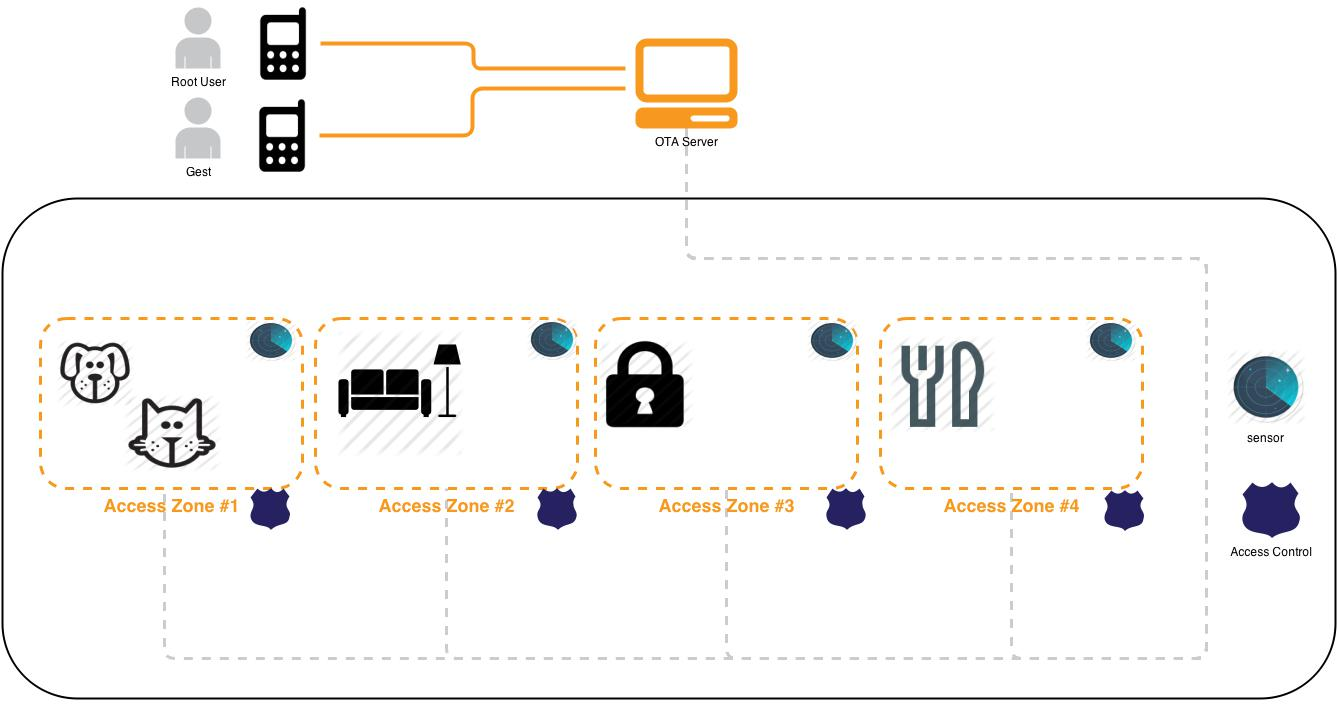
\includegraphics[width=1\textwidth]{homeoverview.jpg}
		\caption{Smart Home}
	\label{fig:SmartHome}
\end{figure}

\section{Overview}
Figure~\ref{fig:SmartHome} describes the basic structure and functionalities provided by implementation scenario Smart Home.
In the above-mentioned housing scenario, embedded with UICC smart card sensors which are in charge of monitoring and reporting environment variables, such as, home temperature, luminance and how much water the pet has, as well as embedded UICC smart card electronic device, for instance coffee maker, are deployed. On each this sensor and device an OPC UA server is installed, whose major responsibilities are controlling that corresponding device as well as managing data gathered by it.  Moreover each door in this scenario is equipped with a digital lock, that only allows user with enough authority to access. This electronic lock is also integrated with a smart card and installed the OPC UA server application. Users in this scenario can be householder or guests of home owner. Using cell phone and on this mobile terminal installed OPC UA client application, subscriber is capable of configuring sensors and querying data gathered by sensors, remote controlling aforementioned secure devices, viewing historical information recorded by corresponding facilities. With the help of such services a comfortable living condition is created in an automated way.  Moreover the root user, namely the owner of this house, is also able to assign the permission of accessing particular room to other guests. In case of when he is taking a vocation, his pet cannot get necessary care.


In this implementation scenario, OPC UA clients, namely Universal Integrated Circuit Card (UICC)  based phone user communicates with OPC UA server, which is deployed on other secure hard devices, via an OTA server.   Smart card that is applied in this scenario acts as security token for both OPC UA client and server and it contains credential information like encryption keys. certificates and digital signature. The communication stack, that manages secure  communication between OPC UA client and server application, is also developed and integrated on smart card as a Java Card applet, which means without smart card and on card Applet, OPC UA client and server are not able to appropriately finish their work.


 \begin{figure}[ht]

	\centering
	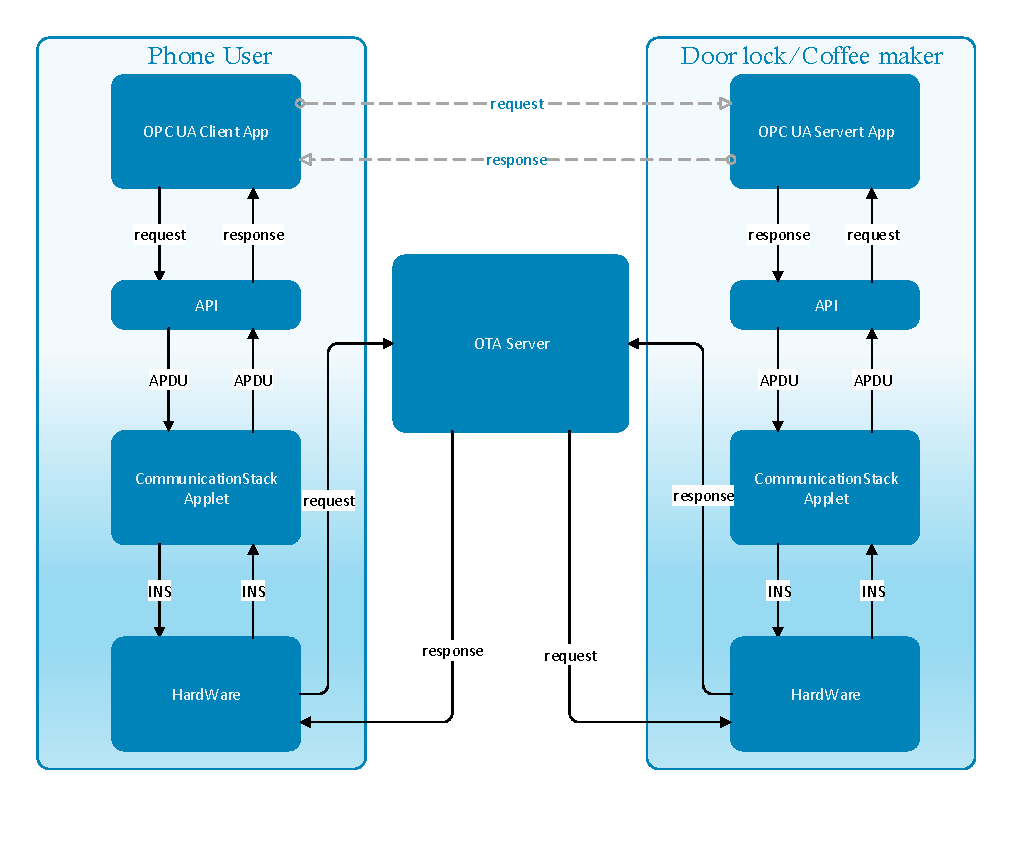
\includegraphics[width=1.1\textwidth]{csoverview}
		\caption{OPC UA Client Server Structure Example}
	\label{fig:softwareStructure}
\end{figure}


\section {Software Structure}

With inspiration offered by application case from section~\ref{secAgent}, my demonstration Smart Home system component structure is illustrated in figure. All devices that build the system are generically referred as system components. And Components are composed of three layers. From bottom to top, they are:

\begin{itemize}
\item Physical layer. In this layer electronic devices and facilities are deployed. Alternatively lower level component could be also in this layer of higher level component.
\item Communication layer. Smart card and OPC UA client/ server application together form this layer. The main responsibility of communication layer is to create a secure communication environment for application layer.
\item Application layer. Different task and hardware specific applications reside in application layer. 
\end{itemize}

Physical layer together with communication layer create a generic platform which supports communication between different hardwares and applications. Moreover this platform also emphasizes the importance of secure messaging, peer authentication as well as authorization and provides corresponding secure mechanisms.

\subsection{Communication Flow}
Figure~\ref{fig:softwareStructure} pictures the communication flow between two system components. OPC UA Client and Server application communicate with each other with the help of an OTA server. And the communication stack is in charge of creation and managing secure communications between OTA server and secure devices. Moreover OPC UA client application is able to communicate with OPC UA server application using Short Message Service(SMS) or TCP/IP based web service. 

When the householder wants to make some coffee, he will send the \emph{makeCoffee} command to coffee maker with his cell phone. And the communication flow between two system components looks like following. Client application installed on cell phone firstly generates the \emph{makeCoffee} request and forwards it to the internal API, which translates the request into APDU and transmits this APDU command to communication stack applet. Communication stack will then creates connection with OTA server and after a successful identification OTA server will confirm the cardholder's identify and forward his request to targeted message receiver. Likewise the request message is going to be transmitted from bottom communication stack to top application step by step. At last the \emph{makeCoffee} command will be performed by coffee maker and a response message is sent back to phone user. 

\subsubsection{Conclusion}\label{secFunction}
In conclusion, server on secure device provides following services:
 \begin{itemize}
  \item processing client subscription/publishing environment data
  \item secure message exchange with client
  \item authority management
  \item historical data record
  \item execution client's command
\end{itemize}
Basic client functions as following are provided:
 \begin{itemize}
  \item submitting subscription/receiving published data
  \item secure message exchange with server
  \item sending command/configuration data
  \item querying system historical data
  \item providing user friendly interface
\end{itemize}

Communication stack is integrated in UICC smart card, whose responsibility is realizing secure channel as well as session management, transporting data to receiver using TCP/IP connections or SMS. An internal API translates OPC UA application instructions in to Application Protocol Data Unity (APDU) messages and forwards them to smart card OS, which is eventually in charge of user authentication and processing secure messaging between card application and chip card pair. 

Moreover thanks to self-containment structure, smart card itself does not dependent on other external resources, which could be extreme vulnerable to potential secure attack, and therefore provides a better hardware security and OS security. 

 \begin{figure}
	\centering
	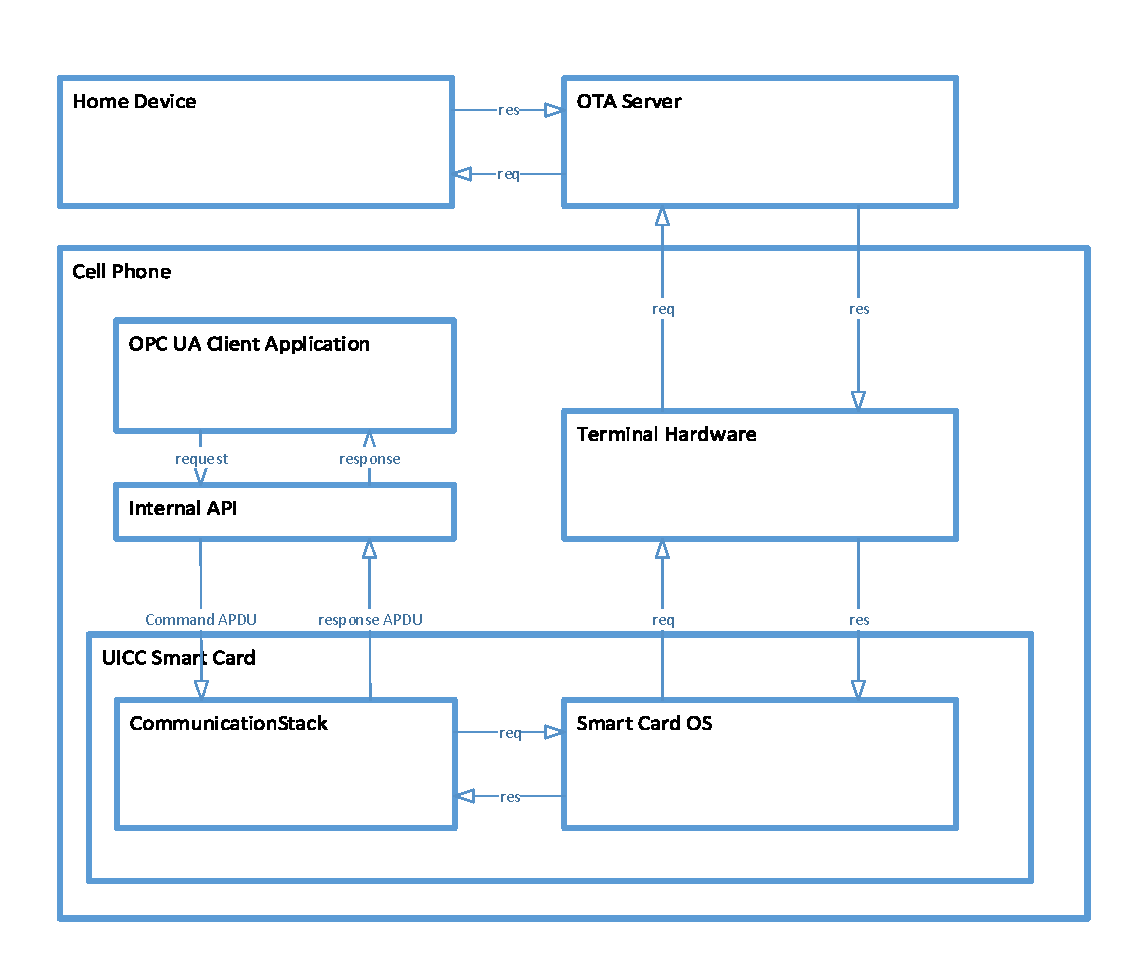
\includegraphics[width=0.78\textwidth]{clientStructure}
		\caption{Client Structure}
	\label{fig:clientStructure}
\end{figure}

\subsection{Client Structure}
As described in figure~\ref{fig:clientStructure}, the OPC UA client consists of client application code that realizes client application level functions, internal API, communication stack applet, smart card and device hardware. The Communication stack's responsibilities are:
\begin{itemize}
  \item initiate HTTP session based on TLS(proactive)
  \item trigger HTTP session based on trigger SMS send by OTA server(passive)
  \item rebuild broken communication channel
  \item message encryption as well as decryption
  \item message transmit
\end{itemize}

\begin{figure}
	\centering
	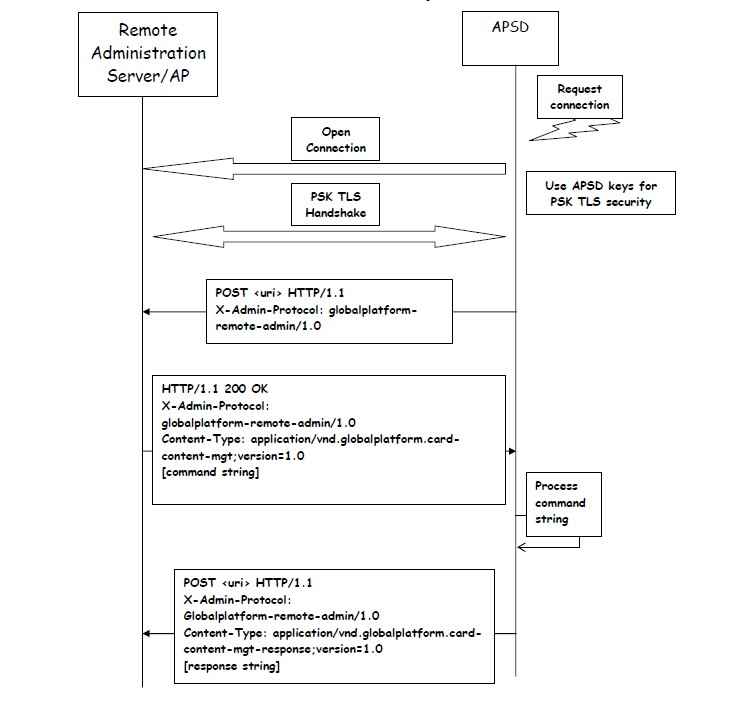
\includegraphics[width=1.2\textwidth]{apsd.jpg}
		\caption{Communication Flow between an AP and corresponding APSD\cite{ramGP}}
	\label{fig:apsd}
\end{figure}
The communication flow compliant with the one provided by GlobalPlatform, which provides mechanisms that allow secure information exchanged between a remote entity and a terminal, this process is also known as Remote Application Management(RAM) over HTTP protocol and PSK TLS security. The on card component, which is responsible for connection creation with the remote entity and user/application authentication, is called Security Domain(SD). And the aforementioned remote entity  is  referred as Remote Administration Server as well. With these concepts, smart card with Security Domain issued  by GloablPlatform can act as HTTP client and is capable of packing APDU formate information into HTTP POST message and transmitting HTTP message to OTA server, which will then forward this HTTP message to target receiver.\cite{ramGP}
 
Figure~\ref{fig:apsd} illustrates a typical communication flow between administration server and corresponding security domain (Application Security Domain) on smart card. As can be seen, the request for open communication is usually initialized by security domain, which is also the phone user. After a successful creation of secure handshake, the remote administration server and security domain are able to based on HTTP connection exchange request and response strings, which encapsulate APDU instructions. GlobalPlatform has also provided  a lists of API used to initialize authentication process, to configure algorithm and keys for message encryption and decryption, to perform secure messaging and etc.

\subsection{Server Structure}

\begin{figure}
	\centering
	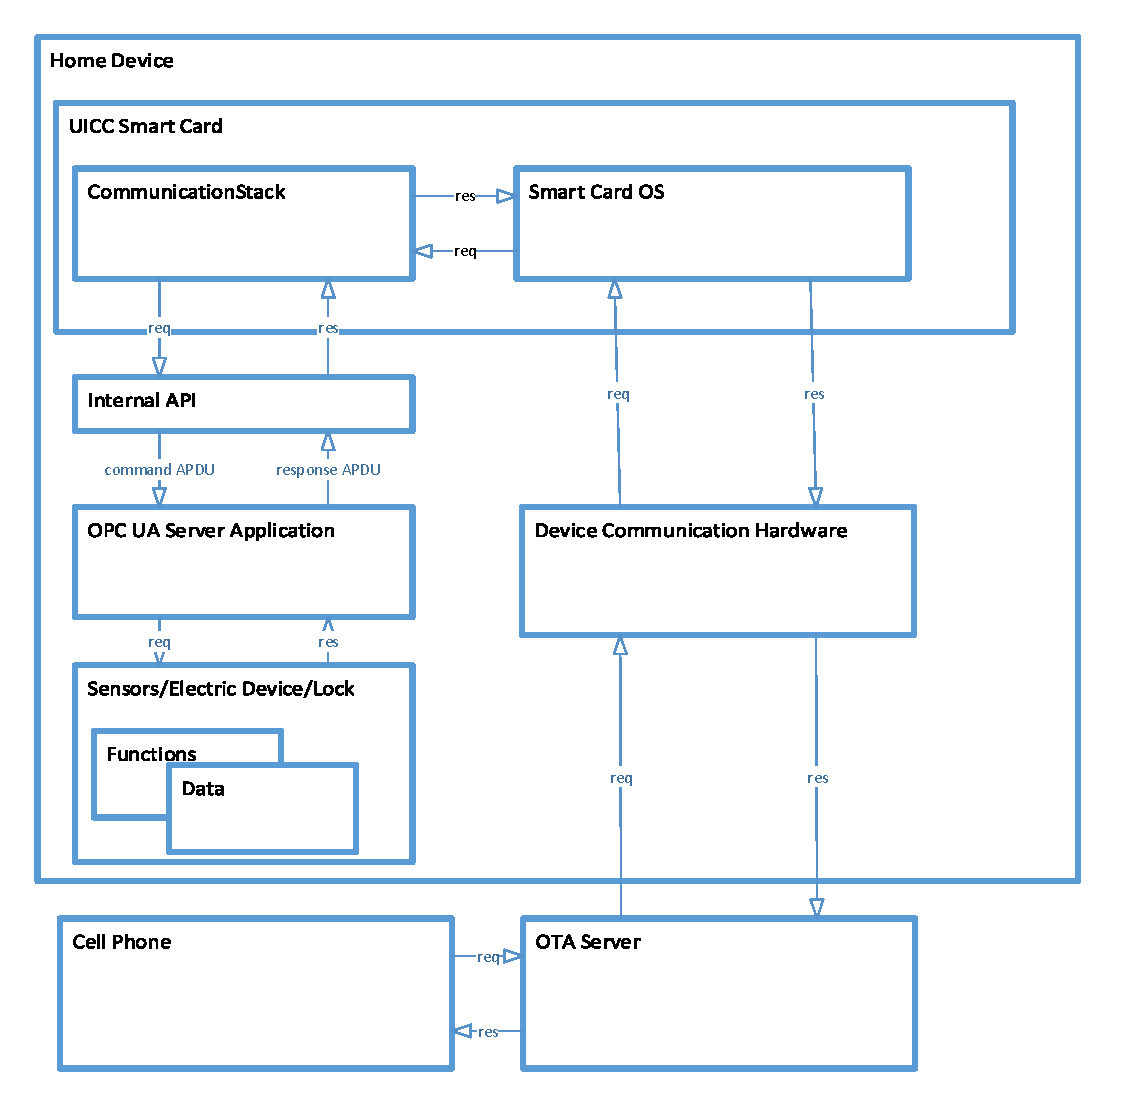
\includegraphics[width=0.95\textwidth]{serverStructure}
		\caption{Server Structure}
	\label{fig:serverStructure}
\end{figure}
Server here refers sensors, electric device as well digital locks that together build up the smart home system. Each server controls exactly one above-mentioned secure device and take subscription as well as publish corresponding notification to authenticated subscriber. The server structure is pictured as figure~\ref{fig:serverStructure} and it consists of OPC UA server application code, which offers basic services like subscription and notification mentioned before, an internal API, an on smart card integrated communication stack and functions as well as data provided by corresponding facility.

\subsection{Implementation Tool Support}
\subsubsection{Java Card Application Design and Debug Tool}
Morpho presents JACADE with full name, Java Card Applet Develop Environment, which is more than just a IDE but a complex selection of various class APIs and software modules, that can be applied to design complete Java Card Applet as well as to debug Java source. 
\subsubsection{Java Card Applet Testing Environment}
When it comes to running test with Java Card Applet, tester has two options. Firstly, he can install the to be tested Applet on a smart card and then connection this chip card with test computer using \emph{Morpho Card Reader (MCR)}. Alternatively \emph{Java virtual card} which is integrated test Applet also could be applied. 

In either way, as next step \emph{Universal Test Environment (UTE)} will be applied. \emph{UTE} provided by Morpho uses Java languages developed test cases
 and test scenarios\footnote{Test scenario is a collection of relative test cases.} to simulate desired use cases and observe corresponding smart card reactions. With the observed test result, tester will be able to analyze Applet's performance and debug corresponding application code. For instance \emph{UTE} can integrate software models used to simulate security domain offered by \emph{Globalplatform} and perform the sophisticate user authentication simulation process.
\subsubsection{Android Application Design Tool}
Eclipse IDE for Java Developer of version 3.7.1 is applied ,together with Android SDK \emph{seek-for-android} and ADT plug-in, as Android Application development environment. Android 2.3.5 is simulated and chosen as demonstration platform.
\subsubsection{Smart Home Simulation Environment}
In order to simulate data manged by home electronic device, \emph{MySQL} database is introduced. And together with \emph{PHP of version 5.5.12}, \emph{Apache of version 2.4.9}, the web server for Smart Home is created. Android Application from previous subsection will then communication with this web server for the purpose of scenario demonstration.